\section{Methodology for Photogrammetric Surveys}
The proposed methodology for automatic photogrammetric surveys with fixed-wing UAV's consists of 4 steps: Mission planning, system integration, execution and processing. Each of those phases includes several steps. The general methodology diagram can be found in figure \ref{fig:methodology_Flow}.
The following section will present a detailed description all the stages and their internal steps
\begin{figure}[H]
\centering
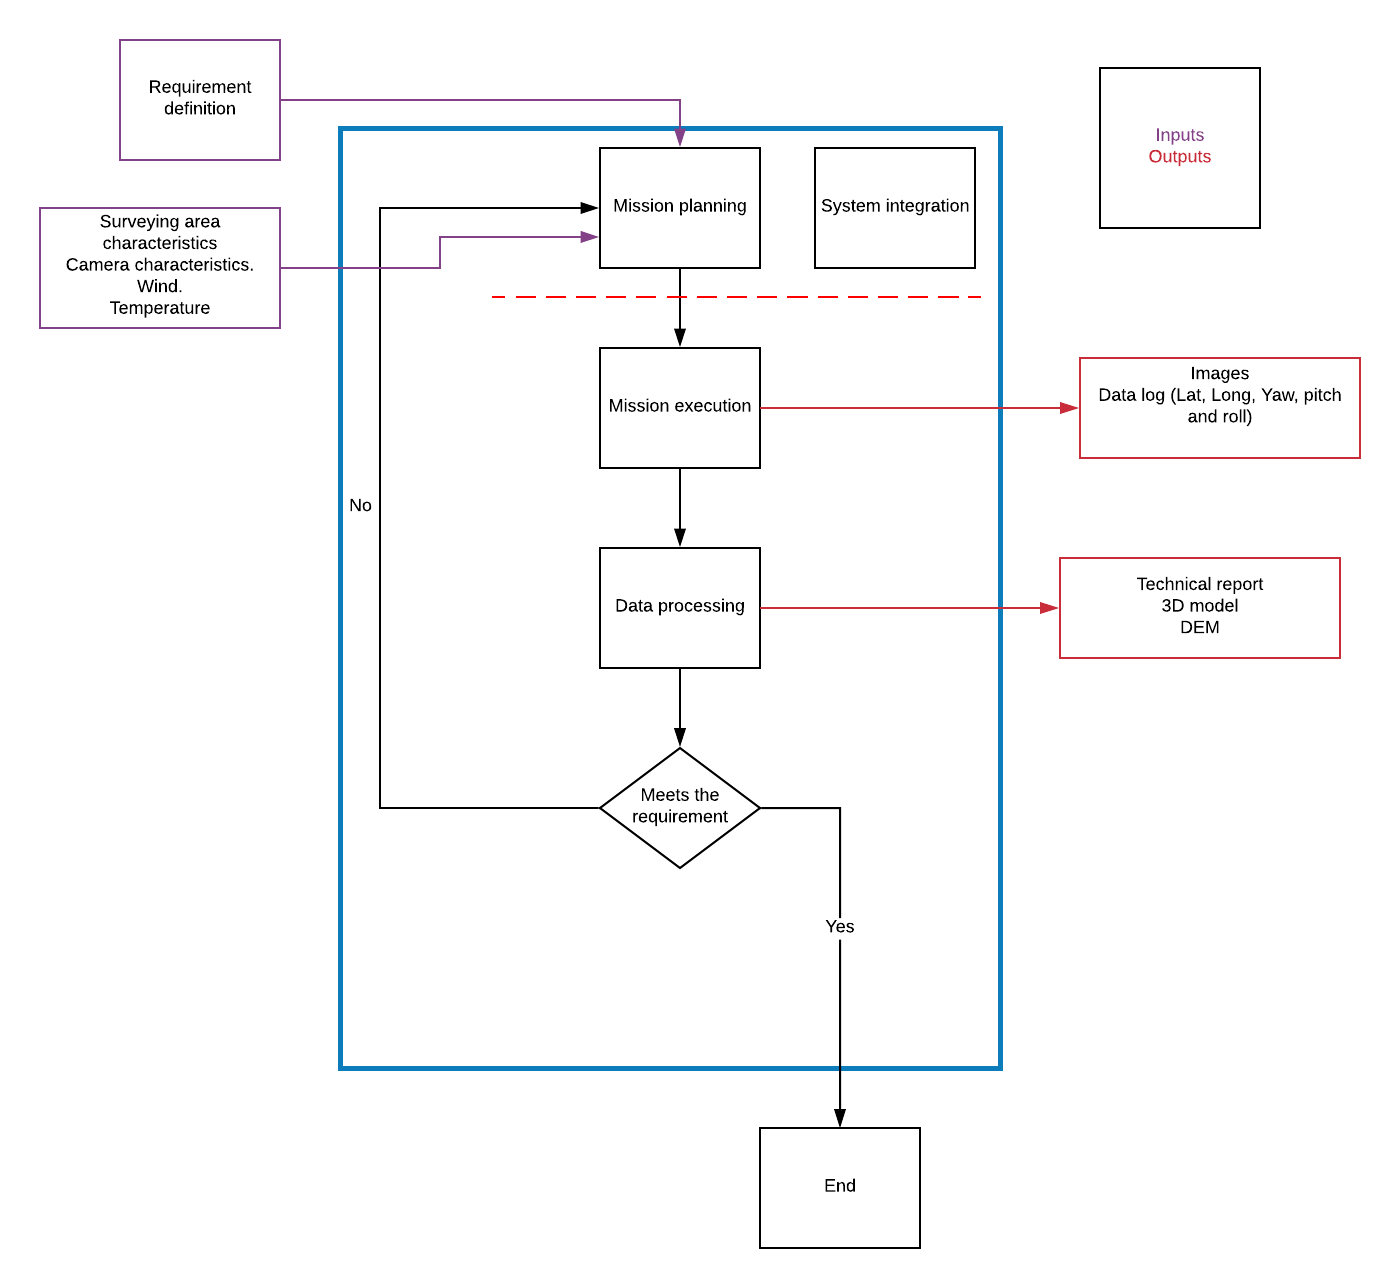
\includegraphics[width=16cm,height=16cm,keepaspectratio]{imagenes/Methodology.png}
\caption{Methodology flow overview}
\label{fig:methodology_Flow}
\end{figure}

This section will give a general overview of each module of the methodology, stating their objective, inputs and outputs.

\subsubsection{Mission planning}
Combining the user requirements, camera characteristics, surveying area, and atmospheric condition, the mission planning module computes and defines parameters used to design the mission path.


\textit{\textbf{Objective:}} Computation and definition of mission design parameters.

\textit{\textbf{Inputs:}} 
\begin{itemize}
    \item Front overlap.
    \item Side overlap.
    \item GSD.
    \item Surveying area.
    \item Camera characteristics.
    \item Surveying area characteristics.
    \item Wind condition.
    \item Temperature.
    \item Sweep angle.
\end{itemize}

\textit{\textbf{Outputs:}} 
\begin{itemize}
    \item Flight path design program:\begin{itemize}
        \item Distance between photos.
        \item Distance between strips.
        \item Number of photos per stripe.
        \item Number of photos for all the mission.
        \item Flight altitude.
    \end{itemize}
    \item Flight limitations.
    \item Simulation.
\end{itemize}
\subsubsection{System integration.}
In this module, the system integration takes place; two main tasks are to be performed in this stage, the first one software integration, then hardware integration.


\textit{\textbf{Objective:}} Integrate the payload to the UAS system, enabling remote controlled operation.

\subsubsection{Mission execution}
Once the mission has been designed and programmed into the UAV is time to execute the flight. This module uses as inputs the outputs of the previous module. The outcome of this module are the images and data log file containing: altitude, longitude, latitude, and attitude information of each picture.

\textit{\textbf{Objective:}} Using the design parameters defined in the planning module, the flight is executed to gather the necessary data.

\textit{\textbf{Inputs:}} 
\begin{itemize}
    \item Flight path design program.
    \item Program files.
\end{itemize}

\textit{\textbf{Outputs:}} 
\begin{itemize}
    \item Pictures
    \item Data log:\begin{itemize}
        \item Latitude.
        \item Longitude.
        \item Yaw.
        \item Pitch.
        \item Roll.
    \end{itemize}
\end{itemize}

\subsubsection{Data processing}
Using  Agisoft Photoscan software to performs the image proccessing, construction of digital elevation models DEM, generation of technical reports, as well as a 3D model from photographs.

\textit{\textbf{Objective:}} Generate a 3D model and DEM using a set of geo-referenced images, perform the photo-alignment, generate the dense point cloud.

\textit{\textbf{Inputs:}} 
\begin{itemize}
    \item Geo-referenced images.
    \item Attitudes and GPS log.
\end{itemize}

\textit{\textbf{Outputs:}} 
\begin{itemize}
    \item Photogrammetric products.
    \begin{itemize}
        \item Report.
        \item DEM.
        \item Otrhmosaic.
    \end{itemize}
\end{itemize}
The next section presents a detailed explanation of the execution of each module of the methodology.
\subsection{Mission Planing}
The first step of the methodology for a photogrammetric mission is the mission planning module, figure \ref{fig:MissionModule} shows an insight into the module flow.
\begin{figure}[H]
\centering
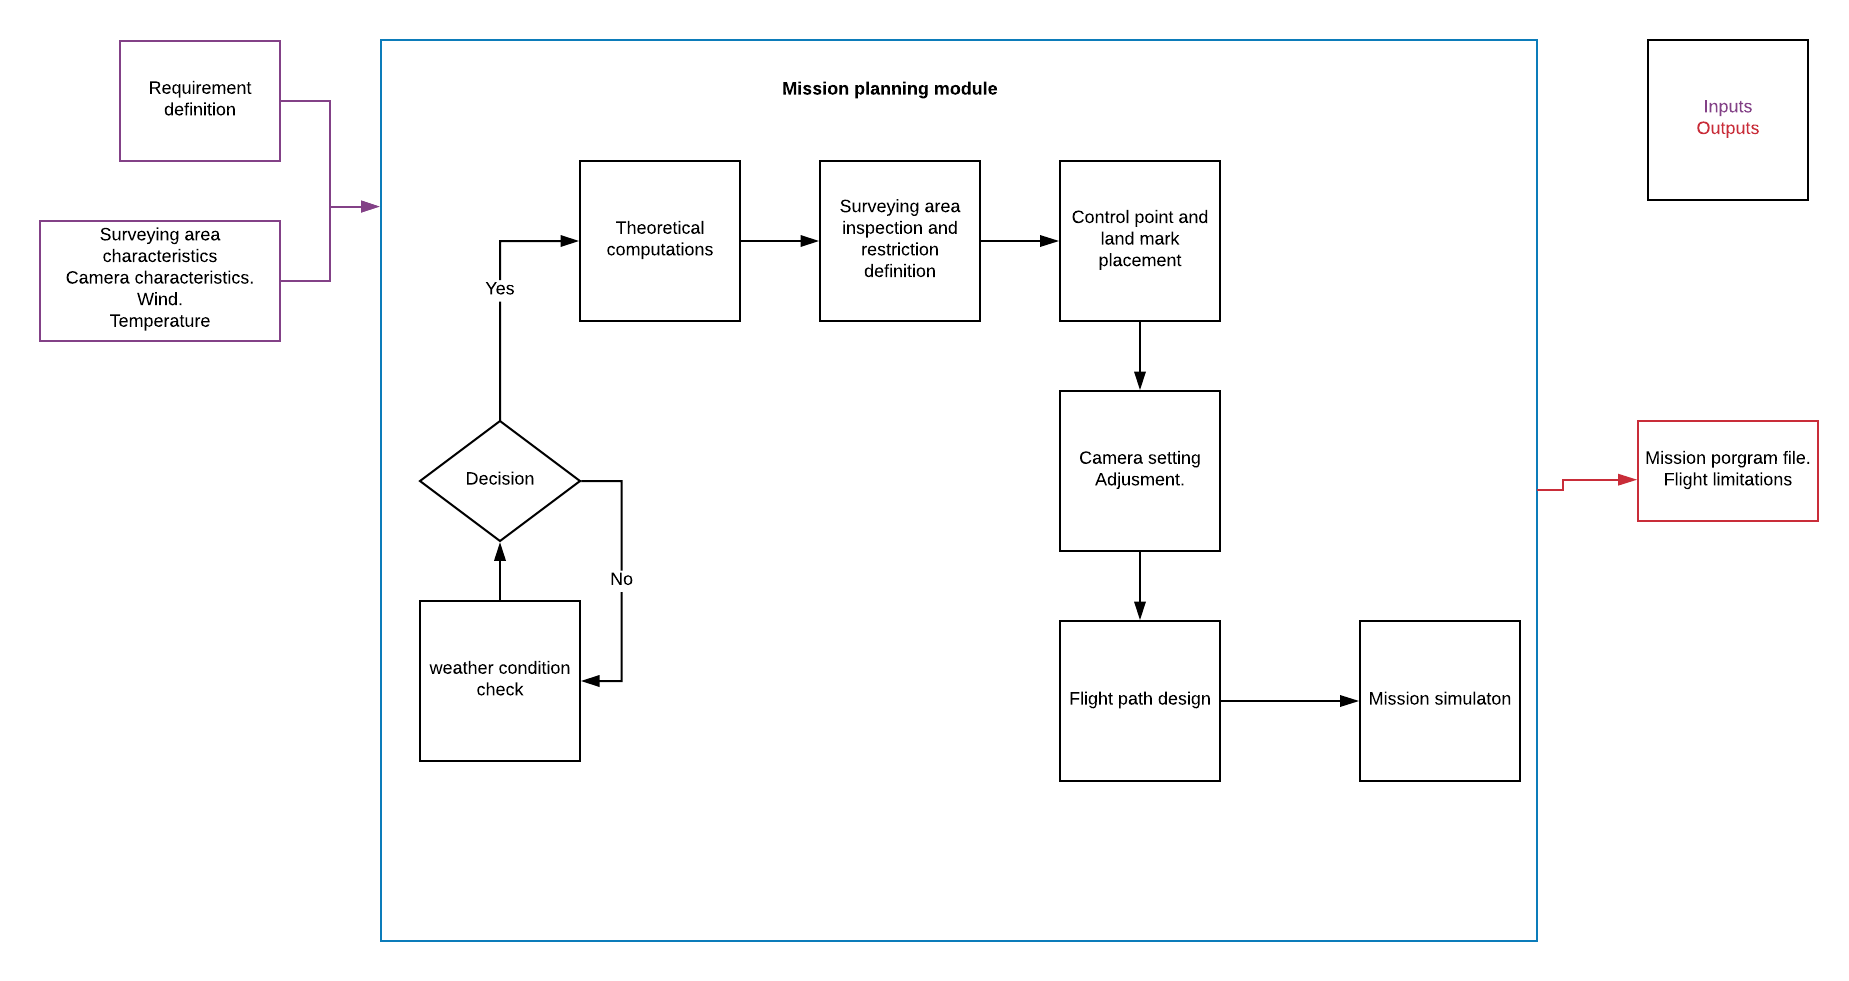
\includegraphics[width=16cm,height=16cm,keepaspectratio]{imagenes/Missionplanning.png}
\caption{Insight into the mission planning module}
\label{fig:MissionModule}
\end{figure}
This module provides all the necessary parameters for a photogrammetric mission with predefined parameters and requisites. The first step is the \textit{atmospheric condition check}. The execution of a photogrammetric mission is limited to a set of weather conditions, that need to be taken into consideration because UAS systems should not operate under an adverse condition such as rain, heavy winds or fog due to safety and law concerns. If the climate requirements for the mission are not met, the task should be postponed.

\textit{\textbf{Theoretical computation}} of the distance between images and distances between continuous strip provide the user with an initial overview of the scope of the mission and result quality. Using the \textit{Matlab} program, the flight parameters are obtained.

\textit{\textbf{The surveying area inspection and restriction}} module the user defines the interest area, taking in consideration factors such as obstacles that may restrict certain maneuvers or procedure. At this point, it is critical to comply with local law and regulation. Depending on the requirements of the photogrammetric product the use of ground control points (GCP) with millimetric precision may be necessary. GCP usually is measured with an RTK system.

\textit{\textbf{Camera adjusment}}\newline
The configuration of before each flight, some of the adjustment parameters are the file format, ISO value, speed of the shutter and lens opening. The adjustments are made with the UAV on the ground.

\textit{\textbf{Mission planning}} is done at the Paparazzi Ground control station and executed in the Apogee flight controller. These allow for the automation of the flight, ensuring a correct flight path through the area, at a stable height and speed, in contrast to the manual mode where errors can be induced when carrying out the trajectory through the path. 

Before entering the execute stage of the methodology is essential to simulate the mission to ensure the correct behavior of the UAV  at moments, taking particular attention to the UAV so it will not exceed its flight capabilities. In the stage, the landing procedure should also checked.
\subsection{System integration.}
The module is divided into two stages that are dependent one from the other: hardware integration and software integration. Figure \ref{fig:Systemintegration} shows an overview of this module.
\begin{figure}[H]
\centering
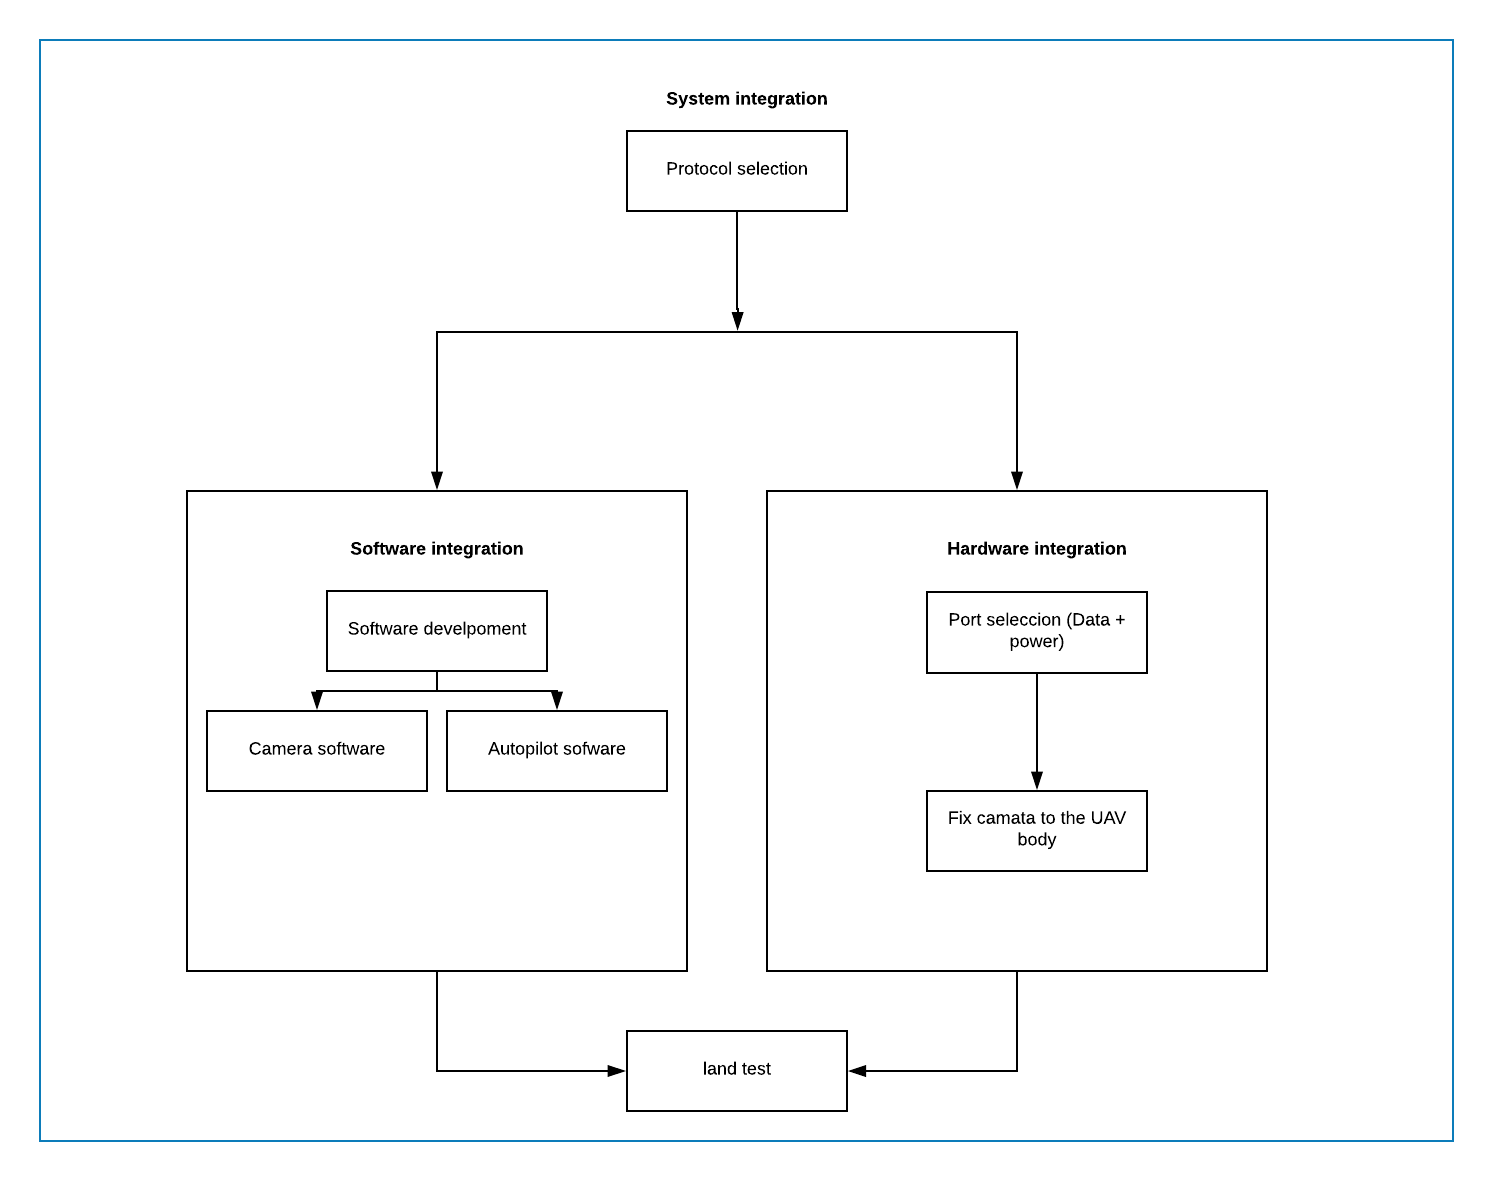
\includegraphics[width=15cm,height=15cm,keepaspectratio]{imagenes/Systemintegration.png}
\caption{System integration module overview}
\label{fig:Systemintegration}
\end{figure}
\textit{\textbf{Protocol selection}}\newline
The first and most crucial step in this module is to identify which ports are available both in the payload (camera) and the autopilot. Usually,  cameras are controlled with PWM signal, either by a physical port o over an IR LED; also some cameras have an UART port that can be used for the interface. 

After the protocol is defined, the module has two parallel tasks that need to be executed: software integration and hardware integration.
\begin{itemize}
    \item \textbf{\textit{Software integration:}} having selected the protocol, the next step is to adapt or develop the necessary software both for the autopilot and the camera. In this stage, requires the design of the "message " or command that the autopilot will send to the camera. In some cases, it will be necessary to develop software capable of prasing the port to obtain such data.
     \item \textbf{\textit{Hardware integration:}} The first action to execute in the hardware section, is to select the power and data port that will be used to connect the camera; usually autopilots have several types of I/Os, for example, servo ports, UART, I2C or SPI. If the power source of the camera is the autopilot, it is essential to make sure that the power requirements are met for both devices.
     
With the physical connection taken care of, the next assignment is to fix the camera to the UAV body. Regularly the commercial UAVs have predefined cutouts to place a camera. When selecting the position, it is critical to make sure that the payload is securely fixed so that it will not move during the mission.
     
\end{itemize}
\textit{\textbf{Land test:}} It is crucial to make sure that the system is working correctly before executing a mission. Thus the last section of this module is to conduct ground testing.

\subsection{Execution}
In this module the flight take place, but before flying it is necessary to take specific steps to ensure the UAV is in the right condition to perform the mission. These steps are explained in this section.  Figure \ref{fig:execute} shows an insight into the module flow.
\begin{figure}[H]
\centering
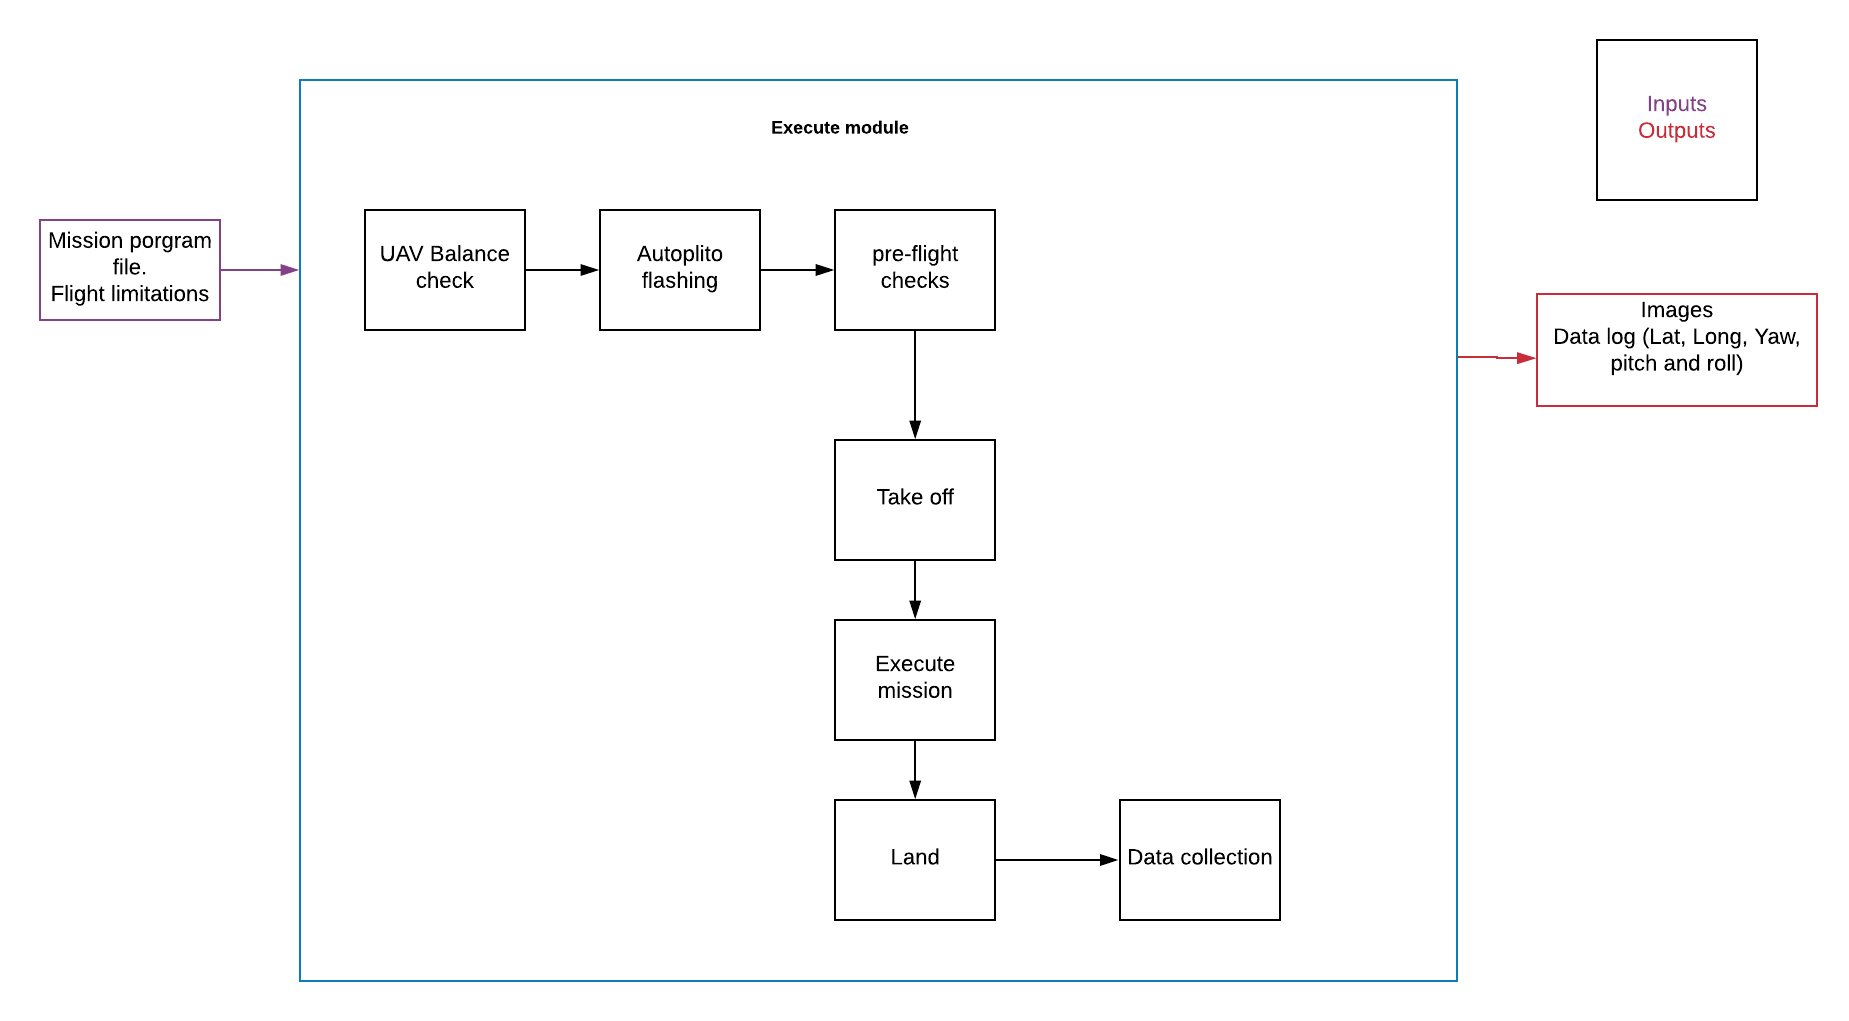
\includegraphics[width=16cm,height=16cm,keepaspectratio]{imagenes/Execution.png}
\caption{Insight into the Execution module}
\label{fig:execute}
\end{figure}
\textit{\textbf{Balance check}} \newline
Correctly balancing the UAV is essential for safe flying, because an incorrect Centre of Gravity (CG or CoG) can potentially result in the plane being quite uncontrollable. Every UAV has a specific CG position; it's the mean point where all gravitational forces act upon the UAV and the point where the plane balances fore-aft correctly. The CG point is determined during the design stage of the UAV or aircraft and is typically shown on a plane as a disc split into four quadrants.

\textit{Balancing procedure} Place the tips of your index or middle fingers under each wing, precisely on the line of the CG. Gently lift the UAV, so it is clear of any surfaces and let it rest freely on your fingertips.
A correctly balanced UAV, sitting on your fingertips, will either be level or have the nose pointing slightly downwards. If the tail looks downwards, then the plane is tail heavy, and readjustment is necessary. Figure \ref{fig:Balance} shows the correct balancing of a UAV.

\begin{figure}[H]
\centering
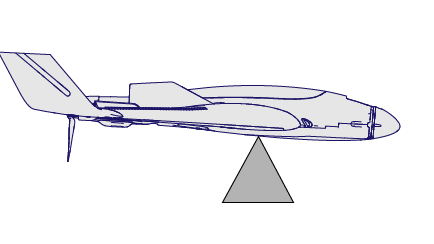
\includegraphics[width=8cm,height=8cm,keepaspectratio]{imagenes/Balance.png}
\caption{Correct UAV Balance}
\label{fig:Balance}
\end{figure}
\textit{\textbf{Pre-flight checks}} \newline
The purpose of pre-flight checks are to ensure that the UAV is in a fit condition to fly and that all systems is working as they should be.  Neglecting to carry out the pre-flight checks can it is likely to result in a crash.. 

\textit{\textbf{Take off}} \newline
Hand launching a big size UAV is teamwork consisting of two persons: The pilot and the thrower. As for a takeoff, a hand launch needs to be done into the wind to maximize the lift under the wings, as well as the airflow over the control surfaces.
The thrower needs to hold the UAV over his head, while the pilot handles the transmitter. When the pilot is ready, he gives the signal to the thrower to start running until the UAV has enough lift. It is crucial to launch firmly, so that stalling speed is avoided when it leaves the thrower hands. 
It is also important to try and keep the UAV level, and do not point it upwards. Trying to lunch in a very nose-up attitude is likely to stall and a crash.

\textit{\textbf{Mission execution}} \newline
The most crucial stage of the module is the execution of the mission. While the plane is in a fully autonomous mode, using the GCS, the user commands the UAV to start the sweep to gather the data.

\textit{\textbf{Landing}} \newline
Once the UAV finishes sweeping the area, the next task to perform is a safe landing. The complete landing circuit is: flying a crosswind leg, turn on to a downwind leg, then a base leg before turning the plane back into the wind and onto final approach. Figure \ref{fig:Landing} illustrates this circuit.
\begin{figure}[H]
\centering
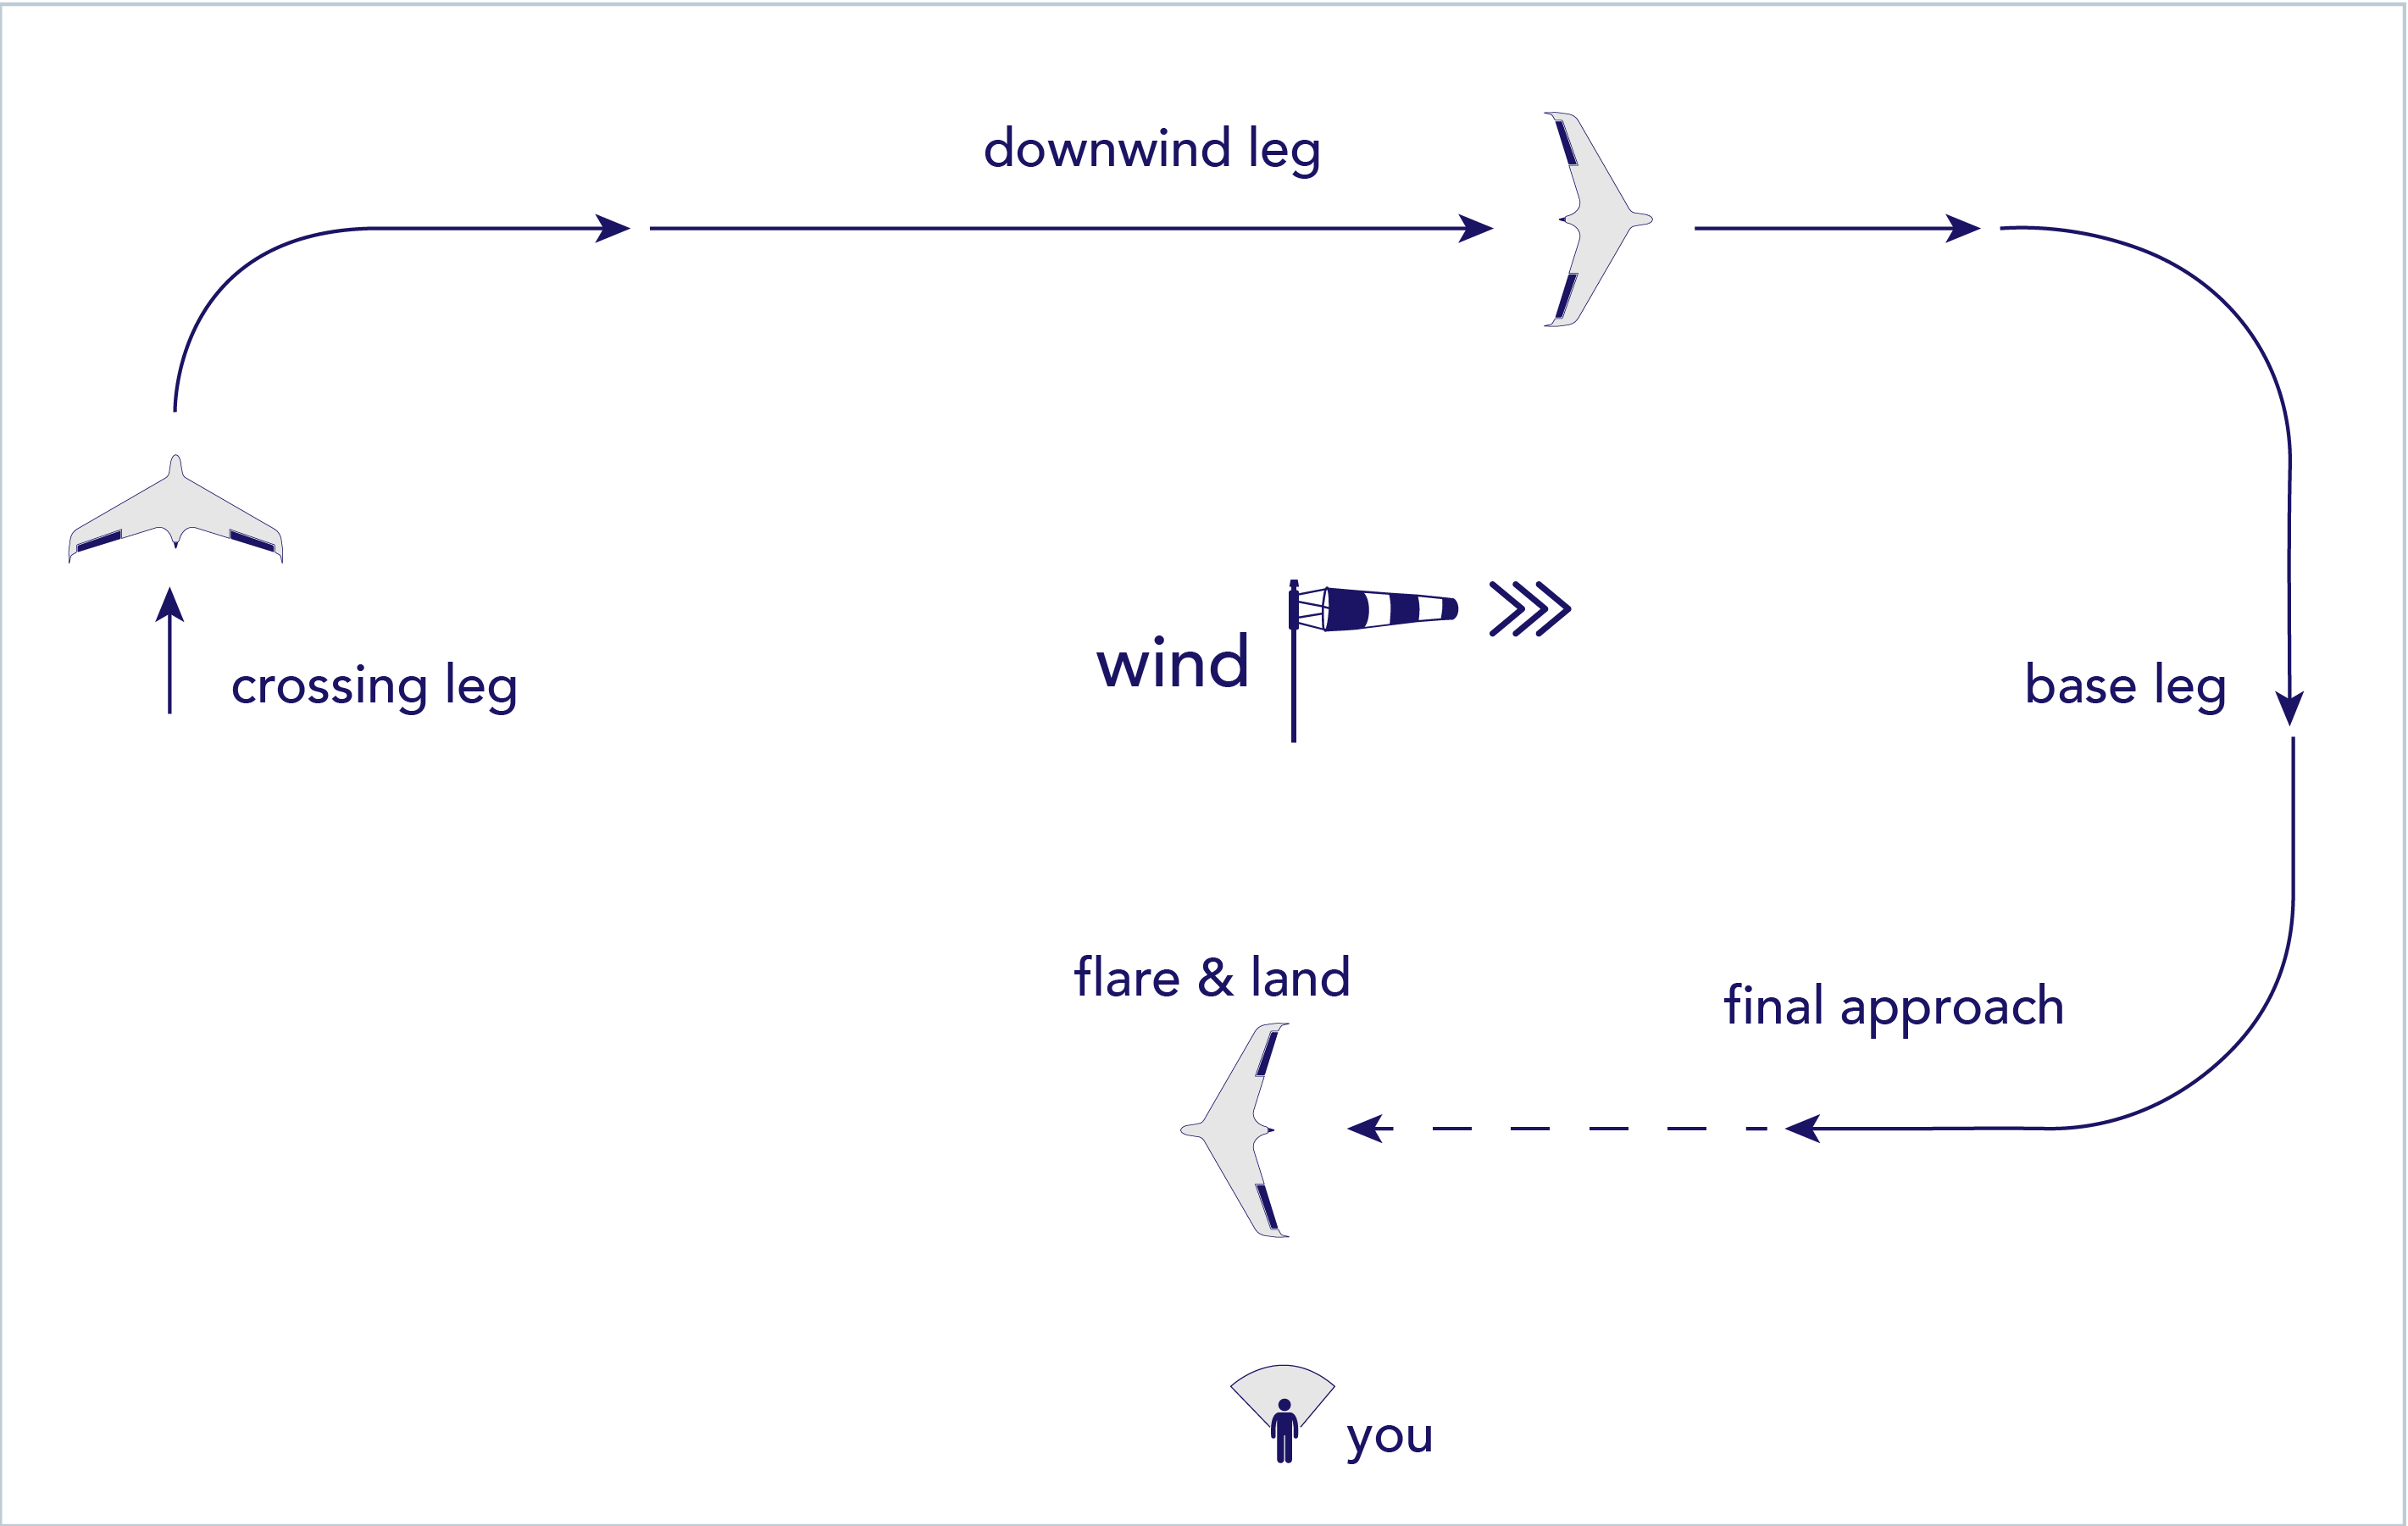
\includegraphics[width=12cm,height=12cm,keepaspectratio]{imagenes/secuencia-aterrizaje-01.png}
\caption{Landing sequence}
\label{fig:Landing}
\end{figure}

\textit{\textbf{Data colletion}} \newline
Once the UAV lands the first thing to do is to disconnect the batteries, the is a critical safety measure, once the power source is detached, it is possible to retrieve the data stored in the camera and the autopilot for further processing. 

\subsection{Processing}
The primary objective of the processing module is, by utilizaing Agisoft software Photoscan, perform the construction of the digital elevation model generating reports, as well as a 3D model from photographs. Figure \ref{fig:DataProcessing} shows the general flow of this module.
\begin{figure}[H]
\centering
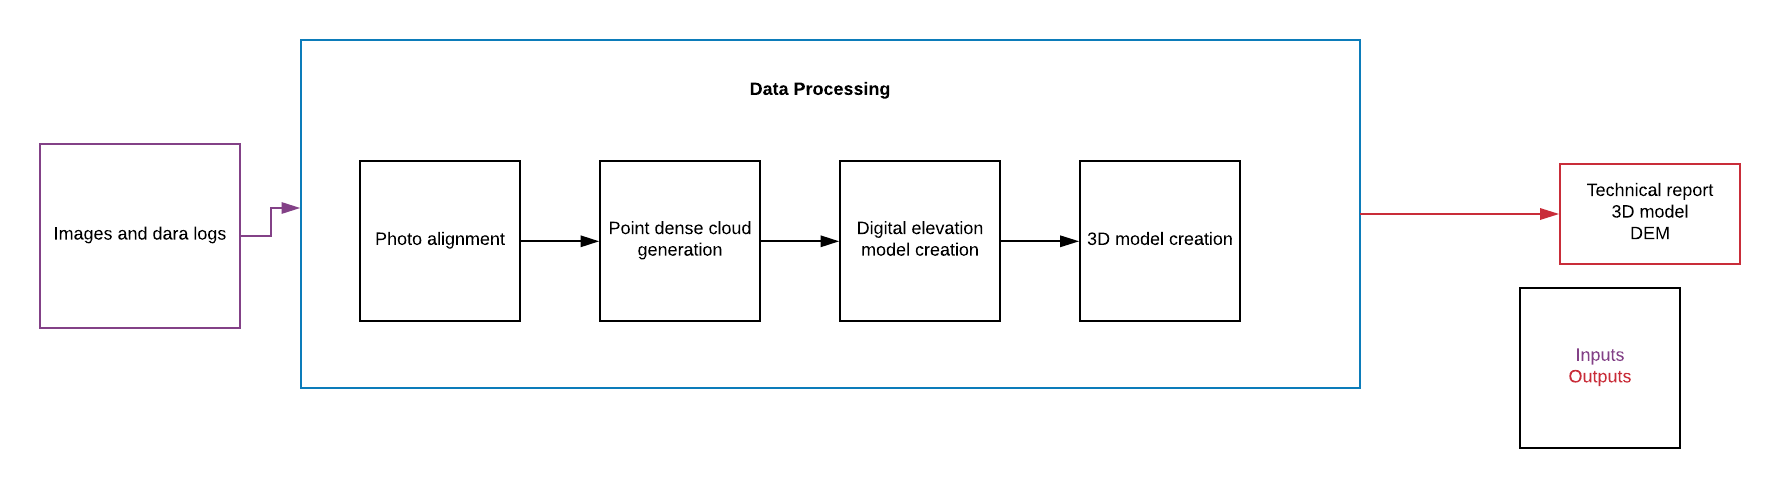
\includegraphics[width=12cm,height=12cm,keepaspectratio]{imagenes/DataProcessing.png}
\caption{Data processing module}
\label{fig:DataProcessing}
\end{figure}
The processing module is responsible for generating the 3D model, model of digital elevation from the inputs of the  georeferenced images and  attitude logs.

\textit{\textbf{Photo alignment}} \newline
The processing starts with the alignment of photographs, using several image processing algorithms. The software searches for the position and orientation of each image, generating a sparse cloud of points.

\textit{\textbf{Dense point cloud}} \newline
Before the generation of the point cloud, the alignment and orientation process must have been carried out with the correct projection system according to the location, because various photogrammetric products such as DEMs and orthomosaics depend on the cloud of points 

\textit{\textbf{Digital elevation model creation}} \newline
Generating the digital elevation model allows the representation of a surface with altitude values to characterize a determined area

